\begin{table}[!h]
     \begin{center}
     \begin{tabular}{ c  p{5cm}  p{5cm}  }
     \toprule
      Peer Nagy & Rollen & F�higkeiten \\ 
    \cmidrule(r){1-1}\cmidrule(lr){2-2}\cmidrule(l){3-3}
     \raisebox{-\totalheight}{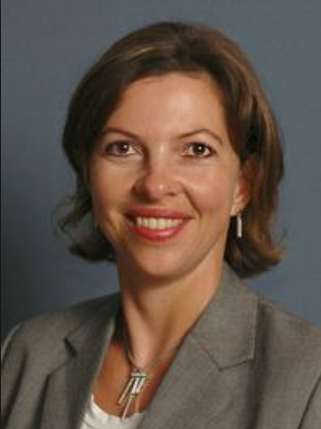
\includegraphics[width=0.2\textwidth]{graphics/Gruppe/2012_Peer_Nagy.PNG}}
      & 
      \begin{itemize}[topsep=0pt] \itemsep0em
      \item Projektleiter
      \item Algorithmuskonzepte erstellen
      \item F\#-Programmierung
      \item Algorithmus\-implementierung
      \end{itemize}
      & 
      \begin{itemize}[topsep=0pt] \itemsep0em
      \item F\#-Kenntnisse
      \item Design
      \item Finanz\-wirtschaftliches Grundwissen
      \end{itemize}
      \\ \bottomrule
      \end{tabular}
      \end{center}
      \end{table}
\begin{table}[!h]
     \begin{center}
     \begin{tabular}{ c  p{5cm}  p{5cm}  }
     \toprule
      Gabriel Pawlowsky & Rollen & F�higkeiten \\ 
    \cmidrule(r){1-1}\cmidrule(lr){2-2}\cmidrule(l){3-3}
     \raisebox{-\totalheight}{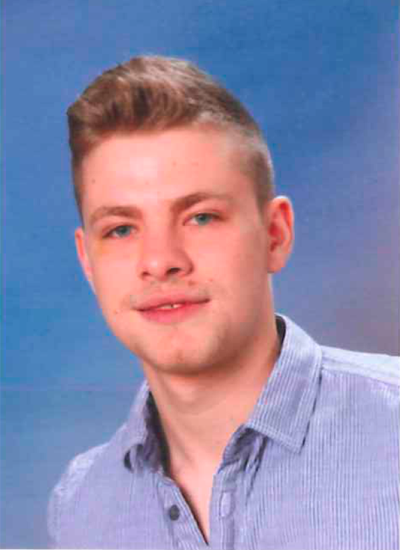
\includegraphics[width=0.2\textwidth]{graphics/Gruppe/2012_Gabriel_Pawlowsky.PNG}}
      & 
      \begin{itemize}[topsep=0pt] \itemsep0em
      \item Stellvertretender \- Pro\-jekt\-lei\-ter
      \item Algorithmus\-kon- \- zept\-be\-rat\-ung
      \item Programmierung der BTS in C\#
      \item Per\-for\-mance\-ana- \- lysen durchf�hren
      \end{itemize}
      & 
      \begin{itemize}[topsep=0pt] \itemsep0em
      \item C\#-Kenntnisse
      \item MS Chart Con\-trols
      \item Algorithmik-Kenntnisse
      \end{itemize}
      \\ \bottomrule
      \end{tabular}
      \end{center}
      \end{table}
\begin{table}[!h]
     \begin{center}
     \begin{tabular}{ c  p{5cm}  p{5cm}  }
     \toprule
      Josef Sochovsky & Rollen & F�higkeiten \\ 
    \cmidrule(r){1-1}\cmidrule(lr){2-2}\cmidrule(l){3-3}
     \raisebox{-\totalheight}{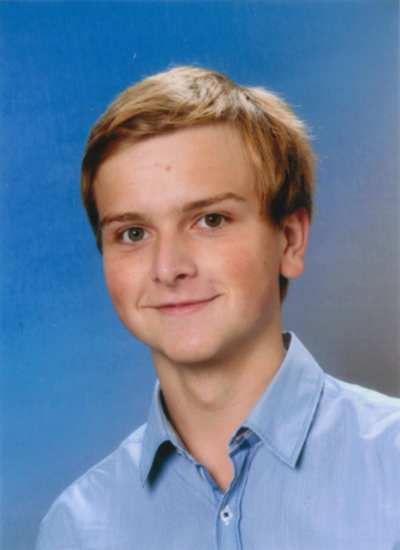
\includegraphics[width=0.2\textwidth]{graphics/Gruppe/2012_Josef_Sochovsky.PNG}}
      & 
      \begin{itemize}[topsep=0pt] \itemsep0em
      \item Technischer Leiter
      \item F\#-Programmierung
      \item Algorithmus\-implementierung
      \item Indikatoren\-implementierung
      \end{itemize}
      & 
      \begin{itemize}[topsep=0pt] \itemsep0em
      \item F\#-Kenntnisse
      \item Algorithmik-Kenntnisse
      \item Finanz\-wirtschaftliches Grundwissen
      \end{itemize}
      \\ \bottomrule
      \end{tabular}
      \end{center}
      \end{table}
